\documentclass{article}

\usepackage[margin=4.00055cm,nohead,a4paper,truedimen,dvips]{geometry}
\usepackage{epic}
\usepackage{eepic}
\usepackage{lscape}
\usepackage{pgfplots}
%\pgfplotsset{compat=newest}
\usetikzlibrary{calc,decorations,decorations.pathreplacing}

\addtolength{\textheight}{-3.65\baselineskip}

\begin{document}

\pagenumbering{gobble}

\author{}
\date{}
\title{}



\newsavebox{\one}
\savebox{\one}{

\scalebox{4}{

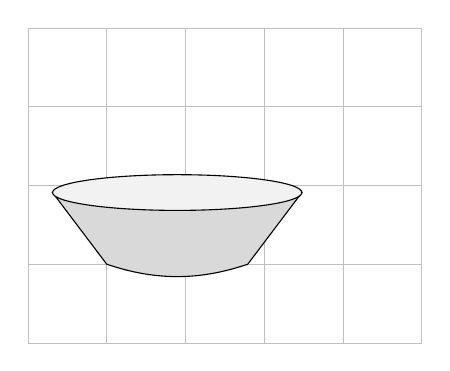
\begin{tikzpicture}

\pgfmathsetmacro{\acoor}{1.95 + random(1,3)*rnd}
\pgfmathsetmacro{\bcoor}{\acoor + rnd}
\pgfmathsetmacro{\ccoor}{.5 + .5*\acoor}
\pgfmathsetmacro{\first}{1 + (.4*\acoor - .5)}
\pgfmathsetmacro{\second}{1 + (.6*\acoor - .5)}
\pgfmathsetmacro{\split}{(2*\bcoor - 1 - \acoor)/2}
\pgfmathsetmacro{\ycoor}{1.5 + 2*rnd}
\pgfmathsetmacro{\corr}{.075 * \ycoor}
\pgfmathsetmacro{\abcorr}{(.08*(\bcoor - 1)) + .0065* \ycoor}


\draw [help lines,lightgray] (0,0) grid (5,4) ;
\draw[fill=gray!30] (1,1) .. controls (\first,1 - \abcorr) and (\second,1 - \abcorr) .. (\acoor,1) -- (\bcoor,\ycoor) --  (1 + \acoor - \bcoor,\ycoor) -- (1,1) ;
\draw[fill=gray!10] (\ccoor,\ycoor) ellipse (\split cm and \split*\corr cm) ;


\end{tikzpicture}
}

}

\newsavebox{\two}
\savebox{\two}{

\scalebox{4}{

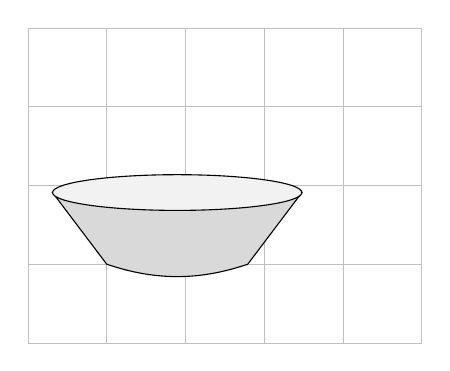
\begin{tikzpicture}

\pgfmathsetmacro{\acoor}{1.95 + random(1,3)*rnd}
\pgfmathsetmacro{\bcoor}{\acoor + rnd}
\pgfmathsetmacro{\ccoor}{.5 + .5*\acoor}
\pgfmathsetmacro{\first}{1 + (.4*\acoor - .5)}
\pgfmathsetmacro{\second}{1 + (.6*\acoor - .5)}
\pgfmathsetmacro{\split}{(2*\bcoor - 1 - \acoor)/2}
\pgfmathsetmacro{\ycoor}{1.5 + 2*rnd}
\pgfmathsetmacro{\corr}{.075 * \ycoor}
\pgfmathsetmacro{\abcorr}{(.08*(\bcoor - 1)) + .0065* \ycoor}


\draw [help lines,lightgray] (0,0) grid (5,4) ;
\draw[fill=gray!30] (1,1) .. controls (\first,1 - \abcorr) and (\second,1 - \abcorr) .. (\acoor,1) -- (\bcoor,\ycoor) --  (1 + \acoor - \bcoor,\ycoor) -- (1,1) ;
\draw[fill=gray!10] (\ccoor,\ycoor) ellipse (\split cm and \split*\corr cm) ;

\end{tikzpicture}
}

}

\newsavebox{\three}
\savebox{\three}{

\scalebox{4}{

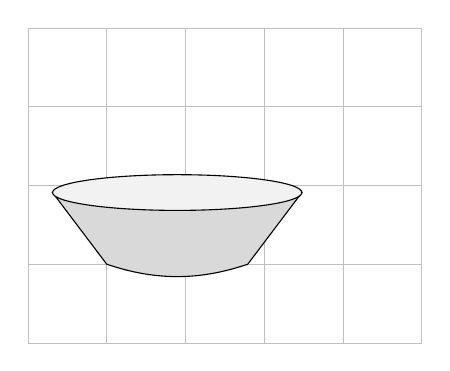
\begin{tikzpicture}

\pgfmathsetmacro{\acoor}{1.95 + random(1,3)*rnd}
\pgfmathsetmacro{\bcoor}{\acoor + rnd}
\pgfmathsetmacro{\ccoor}{.5 + .5*\acoor}
\pgfmathsetmacro{\first}{1 + (.4*\acoor - .5)}
\pgfmathsetmacro{\second}{1 + (.6*\acoor - .5)}
\pgfmathsetmacro{\split}{(2*\bcoor - 1 - \acoor)/2}
\pgfmathsetmacro{\ycoor}{1.5 + 2*rnd}
\pgfmathsetmacro{\corr}{.075 * \ycoor}
\pgfmathsetmacro{\abcorr}{(.08*(\bcoor - 1)) + .0065* \ycoor}


\draw [help lines,lightgray] (0,0) grid (5,4) ;
\draw[fill=gray!30] (1,1) .. controls (\first,1 - \abcorr) and (\second,1 - \abcorr) .. (\acoor,1) -- (\bcoor,\ycoor) --  (1 + \acoor - \bcoor,\ycoor) -- (1,1) ;
\draw[fill=gray!10] (\ccoor,\ycoor) ellipse (\split cm and \split*\corr cm) ;

\end{tikzpicture}
}

}

\newsavebox{\four}
\savebox{\four}{

\scalebox{4}{

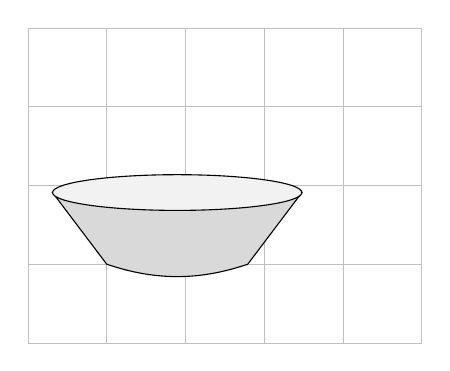
\begin{tikzpicture}

\pgfmathsetmacro{\acoor}{1.95 + random(1,3)*rnd}
\pgfmathsetmacro{\bcoor}{\acoor + rnd}
\pgfmathsetmacro{\ccoor}{.5 + .5*\acoor}
\pgfmathsetmacro{\first}{1 + (.4*\acoor - .5)}
\pgfmathsetmacro{\second}{1 + (.6*\acoor - .5)}
\pgfmathsetmacro{\split}{(2*\bcoor - 1 - \acoor)/2}
\pgfmathsetmacro{\ycoor}{1.5 + 2*rnd}
\pgfmathsetmacro{\corr}{.075 * \ycoor}
\pgfmathsetmacro{\abcorr}{(.08*(\bcoor - 1)) + .0065* \ycoor}


\draw [help lines,lightgray] (0,0) grid (5,4) ;
\draw[fill=gray!30] (1,1) .. controls (\first,1 - \abcorr) and (\second,1 - \abcorr) .. (\acoor,1) -- (\bcoor,\ycoor) --  (1 + \acoor - \bcoor,\ycoor) -- (1,1) ;
\draw[fill=gray!10] (\ccoor,\ycoor) ellipse (\split cm and \split*\corr cm) ;

\end{tikzpicture}
}

}

\newsavebox{\five}
\savebox{\five}{

\scalebox{4}{

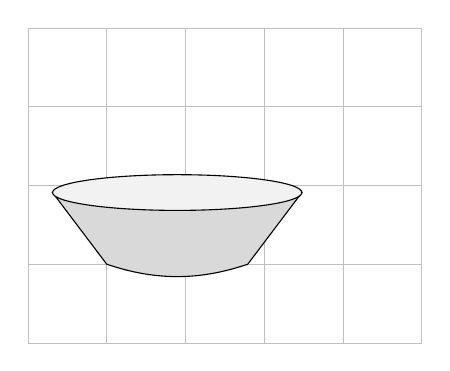
\begin{tikzpicture}

\pgfmathsetmacro{\acoor}{1.95 + random(1,3)*rnd}
\pgfmathsetmacro{\bcoor}{\acoor + rnd}
\pgfmathsetmacro{\ccoor}{.5 + .5*\acoor}
\pgfmathsetmacro{\first}{1 + (.4*\acoor - .5)}
\pgfmathsetmacro{\second}{1 + (.6*\acoor - .5)}
\pgfmathsetmacro{\split}{(2*\bcoor - 1 - \acoor)/2}
\pgfmathsetmacro{\ycoor}{1.5 + 2*rnd}
\pgfmathsetmacro{\corr}{.075 * \ycoor}
\pgfmathsetmacro{\abcorr}{(.08*(\bcoor - 1)) + .0065* \ycoor}


\draw [help lines,lightgray] (0,0) grid (5,4) ;
\draw[fill=gray!30] (1,1) .. controls (\first,1 - \abcorr) and (\second,1 - \abcorr) .. (\acoor,1) -- (\bcoor,\ycoor) --  (1 + \acoor - \bcoor,\ycoor) -- (1,1) ;
\draw[fill=gray!10] (\ccoor,\ycoor) ellipse (\split cm and \split*\corr cm) ;

\end{tikzpicture}
}

}

\newsavebox{\six}
\savebox{\six}{

\scalebox{4}{

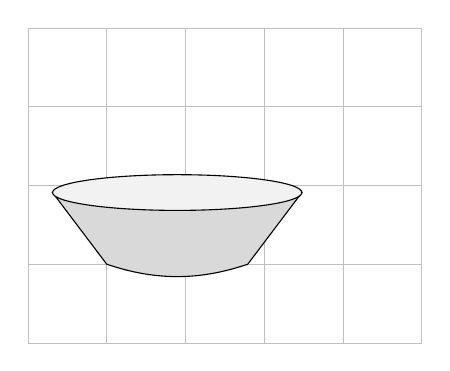
\begin{tikzpicture}

\pgfmathsetmacro{\acoor}{1.95 + random(1,3)*rnd}
\pgfmathsetmacro{\bcoor}{\acoor + rnd}
\pgfmathsetmacro{\ccoor}{.5 + .5*\acoor}
\pgfmathsetmacro{\first}{1 + (.4*\acoor - .5)}
\pgfmathsetmacro{\second}{1 + (.6*\acoor - .5)}
\pgfmathsetmacro{\split}{(2*\bcoor - 1 - \acoor)/2}
\pgfmathsetmacro{\ycoor}{1.5 + 2*rnd}
\pgfmathsetmacro{\corr}{.075 * \ycoor}
\pgfmathsetmacro{\abcorr}{(.08*(\bcoor - 1)) + .0065* \ycoor}


\draw [help lines,lightgray] (0,0) grid (5,4) ;
\draw[fill=gray!30] (1,1) .. controls (\first,1 - \abcorr) and (\second,1 - \abcorr) .. (\acoor,1) -- (\bcoor,\ycoor) --  (1 + \acoor - \bcoor,\ycoor) -- (1,1) ;
\draw[fill=gray!10] (\ccoor,\ycoor) ellipse (\split cm and \split*\corr cm) ;

\end{tikzpicture}
}

}
\newsavebox{\seven}
\savebox{\seven}{

\scalebox{4}{

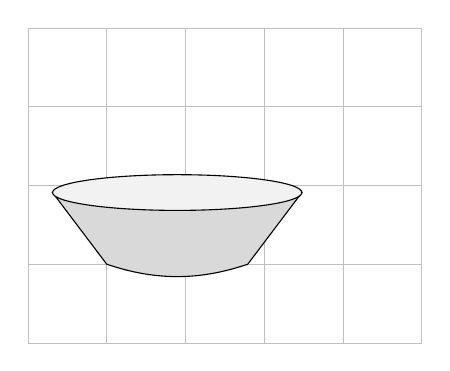
\begin{tikzpicture}

\pgfmathsetmacro{\acoor}{1.95 + random(1,3)*rnd}
\pgfmathsetmacro{\bcoor}{\acoor + rnd}
\pgfmathsetmacro{\ccoor}{.5 + .5*\acoor}
\pgfmathsetmacro{\first}{1 + (.4*\acoor - .5)}
\pgfmathsetmacro{\second}{1 + (.6*\acoor - .5)}
\pgfmathsetmacro{\split}{(2*\bcoor - 1 - \acoor)/2}
\pgfmathsetmacro{\ycoor}{1.5 + 2*rnd}
\pgfmathsetmacro{\corr}{.075 * \ycoor}
\pgfmathsetmacro{\abcorr}{(.08*(\bcoor - 1)) + .0065* \ycoor}


\draw [help lines,lightgray] (0,0) grid (5,4) ;
\draw[fill=gray!30] (1,1) .. controls (\first,1 - \abcorr) and (\second,1 - \abcorr) .. (\acoor,1) -- (\bcoor,\ycoor) --  (1 + \acoor - \bcoor,\ycoor) -- (1,1) ;
\draw[fill=gray!10] (\ccoor,\ycoor) ellipse (\split cm and \split*\corr cm) ;

\end{tikzpicture}
}

}
\newsavebox{\eight}
\savebox{\eight}{

\scalebox{4}{

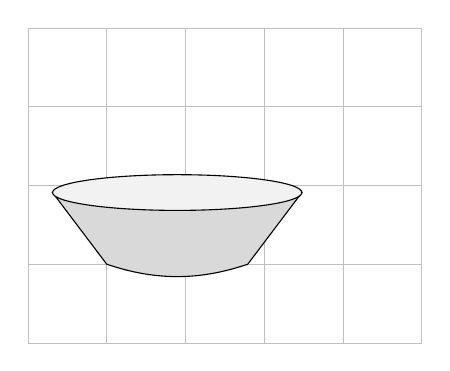
\begin{tikzpicture}

\pgfmathsetmacro{\acoor}{1.95 + random(1,3)*rnd}
\pgfmathsetmacro{\bcoor}{\acoor + rnd}
\pgfmathsetmacro{\ccoor}{.5 + .5*\acoor}
\pgfmathsetmacro{\first}{1 + (.4*\acoor - .5)}
\pgfmathsetmacro{\second}{1 + (.6*\acoor - .5)}
\pgfmathsetmacro{\split}{(2*\bcoor - 1 - \acoor)/2}
\pgfmathsetmacro{\ycoor}{1.5 + 2*rnd}
\pgfmathsetmacro{\corr}{.075 * \ycoor}
\pgfmathsetmacro{\abcorr}{(.08*(\bcoor - 1)) + .0065* \ycoor}


\draw [help lines,lightgray] (0,0) grid (5,4) ;
\draw[fill=gray!30] (1,1) .. controls (\first,1 - \abcorr) and (\second,1 - \abcorr) .. (\acoor,1) -- (\bcoor,\ycoor) --  (1 + \acoor - \bcoor,\ycoor) -- (1,1) ;
\draw[fill=gray!10] (\ccoor,\ycoor) ellipse (\split cm and \split*\corr cm) ;

\end{tikzpicture}
}

}
\newsavebox{\nine}
\savebox{\nine}{

\scalebox{4}{

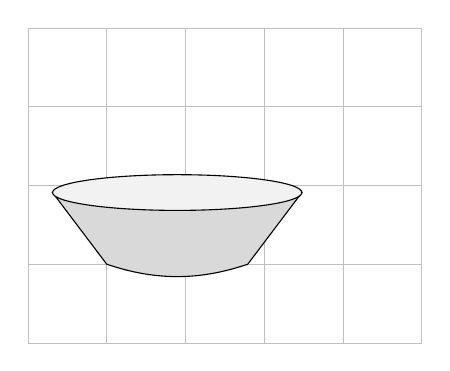
\begin{tikzpicture}

\pgfmathsetmacro{\acoor}{1.95 + random(1,3)*rnd}
\pgfmathsetmacro{\bcoor}{\acoor + rnd}
\pgfmathsetmacro{\ccoor}{.5 + .5*\acoor}
\pgfmathsetmacro{\first}{1 + (.4*\acoor - .5)}
\pgfmathsetmacro{\second}{1 + (.6*\acoor - .5)}
\pgfmathsetmacro{\split}{(2*\bcoor - 1 - \acoor)/2}
\pgfmathsetmacro{\ycoor}{1.5 + 2*rnd}
\pgfmathsetmacro{\corr}{.075 * \ycoor}
\pgfmathsetmacro{\abcorr}{(.08*(\bcoor - 1)) + .0065* \ycoor}


\draw [help lines,lightgray] (0,0) grid (5,4) ;
\draw[fill=gray!30] (1,1) .. controls (\first,1 - \abcorr) and (\second,1 - \abcorr) .. (\acoor,1) -- (\bcoor,\ycoor) --  (1 + \acoor - \bcoor,\ycoor) -- (1,1) ;
\draw[fill=gray!10] (\ccoor,\ycoor) ellipse (\split cm and \split*\corr cm) ;

\end{tikzpicture}
}

}

\newsavebox{\ten}
\savebox{\ten}{

\scalebox{4}{

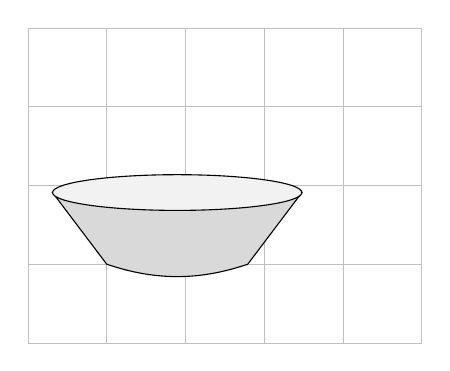
\begin{tikzpicture}

\pgfmathsetmacro{\acoor}{1.95 + random(1,3)*rnd}
\pgfmathsetmacro{\bcoor}{\acoor + rnd}
\pgfmathsetmacro{\ccoor}{.5 + .5*\acoor}
\pgfmathsetmacro{\first}{1 + (.4*\acoor - .5)}
\pgfmathsetmacro{\second}{1 + (.6*\acoor - .5)}
\pgfmathsetmacro{\split}{(2*\bcoor - 1 - \acoor)/2}
\pgfmathsetmacro{\ycoor}{1.5 + 2*rnd}
\pgfmathsetmacro{\corr}{.075 * \ycoor}
\pgfmathsetmacro{\abcorr}{(.08*(\bcoor - 1)) + .0065* \ycoor}


\draw [help lines,lightgray] (0,0) grid (5,4) ;
\draw[fill=gray!30] (1,1) .. controls (\first,1 - \abcorr) and (\second,1 - \abcorr) .. (\acoor,1) -- (\bcoor,\ycoor) --  (1 + \acoor - \bcoor,\ycoor) -- (1,1) ;
\draw[fill=gray!10] (\ccoor,\ycoor) ellipse (\split cm and \split*\corr cm) ;

\end{tikzpicture}
}

}

\newsavebox{\eleven}
\savebox{\eleven}{

\scalebox{4}{

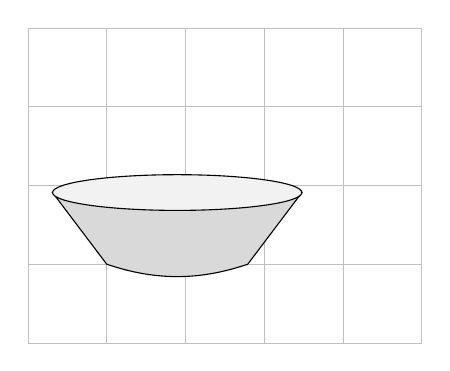
\begin{tikzpicture}

\pgfmathsetmacro{\acoor}{1.95 + random(1,3)*rnd}
\pgfmathsetmacro{\bcoor}{\acoor + rnd}
\pgfmathsetmacro{\ccoor}{.5 + .5*\acoor}
\pgfmathsetmacro{\first}{1 + (.4*\acoor - .5)}
\pgfmathsetmacro{\second}{1 + (.6*\acoor - .5)}
\pgfmathsetmacro{\split}{(2*\bcoor - 1 - \acoor)/2}
\pgfmathsetmacro{\ycoor}{1.5 + 2*rnd}
\pgfmathsetmacro{\corr}{.075 * \ycoor}
\pgfmathsetmacro{\abcorr}{(.08*(\bcoor - 1)) + .0065* \ycoor}


\draw [help lines,lightgray] (0,0) grid (5,4) ;
\draw[fill=gray!30] (1,1) .. controls (\first,1 - \abcorr) and (\second,1 - \abcorr) .. (\acoor,1) -- (\bcoor,\ycoor) --  (1 + \acoor - \bcoor,\ycoor) -- (1,1) ;
\draw[fill=gray!10] (\ccoor,\ycoor) ellipse (\split cm and \split*\corr cm) ;

\end{tikzpicture}
}

}
\newsavebox{\twelve}
\savebox{\twelve}{

\scalebox{4}{

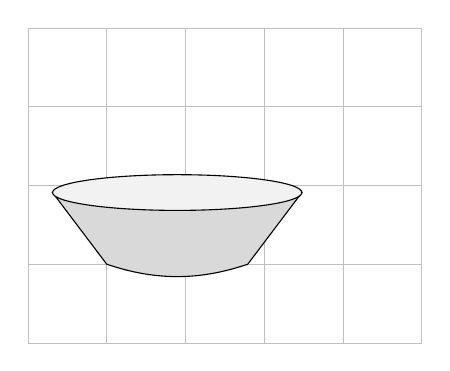
\begin{tikzpicture}

\pgfmathsetmacro{\acoor}{1.95 + random(1,3)*rnd}
\pgfmathsetmacro{\bcoor}{\acoor + rnd}
\pgfmathsetmacro{\ccoor}{.5 + .5*\acoor}
\pgfmathsetmacro{\first}{1 + (.4*\acoor - .5)}
\pgfmathsetmacro{\second}{1 + (.6*\acoor - .5)}
\pgfmathsetmacro{\split}{(2*\bcoor - 1 - \acoor)/2}
\pgfmathsetmacro{\ycoor}{1.5 + 2*rnd}
\pgfmathsetmacro{\corr}{.075 * \ycoor}
\pgfmathsetmacro{\abcorr}{(.08*(\bcoor - 1)) + .0065* \ycoor}


\draw [help lines,lightgray] (0,0) grid (5,4) ;
\draw[fill=gray!30] (1,1) .. controls (\first,1 - \abcorr) and (\second,1 - \abcorr) .. (\acoor,1) -- (\bcoor,\ycoor) --  (1 + \acoor - \bcoor,\ycoor) -- (1,1) ;
\draw[fill=gray!10] (\ccoor,\ycoor) ellipse (\split cm and \split*\corr cm) ;

\end{tikzpicture}
}

}
\newsavebox{\thirteen}
\savebox{\thirteen}{

\scalebox{4}{

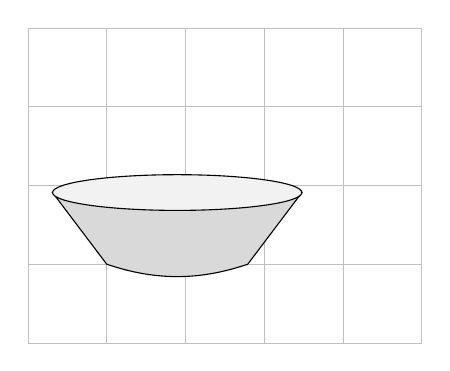
\begin{tikzpicture}

\pgfmathsetmacro{\acoor}{1.95 + random(1,3)*rnd}
\pgfmathsetmacro{\bcoor}{\acoor + rnd}
\pgfmathsetmacro{\ccoor}{.5 + .5*\acoor}
\pgfmathsetmacro{\first}{1 + (.4*\acoor - .5)}
\pgfmathsetmacro{\second}{1 + (.6*\acoor - .5)}
\pgfmathsetmacro{\split}{(2*\bcoor - 1 - \acoor)/2}
\pgfmathsetmacro{\ycoor}{1.5 + 2*rnd}
\pgfmathsetmacro{\corr}{.075 * \ycoor}
\pgfmathsetmacro{\abcorr}{(.08*(\bcoor - 1)) + .0065* \ycoor}


\draw [help lines,lightgray] (0,0) grid (5,4) ;
\draw[fill=gray!30] (1,1) .. controls (\first,1 - \abcorr) and (\second,1 - \abcorr) .. (\acoor,1) -- (\bcoor,\ycoor) --  (1 + \acoor - \bcoor,\ycoor) -- (1,1) ;
\draw[fill=gray!10] (\ccoor,\ycoor) ellipse (\split cm and \split*\corr cm) ;

\end{tikzpicture}
}

}
\newsavebox{\fourteen}
\savebox{\fourteen}{

\scalebox{4}{

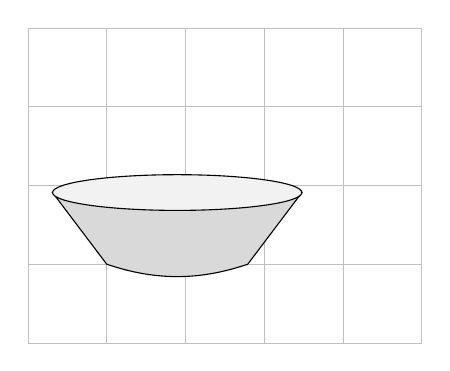
\begin{tikzpicture}

\pgfmathsetmacro{\acoor}{1.95 + random(1,3)*rnd}
\pgfmathsetmacro{\bcoor}{\acoor + rnd}
\pgfmathsetmacro{\ccoor}{.5 + .5*\acoor}
\pgfmathsetmacro{\first}{1 + (.4*\acoor - .5)}
\pgfmathsetmacro{\second}{1 + (.6*\acoor - .5)}
\pgfmathsetmacro{\split}{(2*\bcoor - 1 - \acoor)/2}
\pgfmathsetmacro{\ycoor}{1.5 + 2*rnd}
\pgfmathsetmacro{\corr}{.075 * \ycoor}
\pgfmathsetmacro{\abcorr}{(.08*(\bcoor - 1)) + .0065* \ycoor}


\draw [help lines,lightgray] (0,0) grid (5,4) ;
\draw[fill=gray!30] (1,1) .. controls (\first,1 - \abcorr) and (\second,1 - \abcorr) .. (\acoor,1) -- (\bcoor,\ycoor) --  (1 + \acoor - \bcoor,\ycoor) -- (1,1) ;
\draw[fill=gray!10] (\ccoor,\ycoor) ellipse (\split cm and \split*\corr cm) ;

\end{tikzpicture}
}

}
\newsavebox{\fifteen}
\savebox{\fifteen}{

\scalebox{4}{

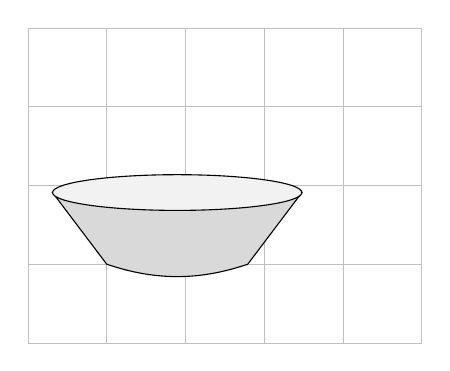
\begin{tikzpicture}

\pgfmathsetmacro{\acoor}{1.95 + random(1,3)*rnd}
\pgfmathsetmacro{\bcoor}{\acoor + rnd}
\pgfmathsetmacro{\ccoor}{.5 + .5*\acoor}
\pgfmathsetmacro{\first}{1 + (.4*\acoor - .5)}
\pgfmathsetmacro{\second}{1 + (.6*\acoor - .5)}
\pgfmathsetmacro{\split}{(2*\bcoor - 1 - \acoor)/2}
\pgfmathsetmacro{\ycoor}{1.5 + 2*rnd}
\pgfmathsetmacro{\corr}{.075 * \ycoor}
\pgfmathsetmacro{\abcorr}{(.08*(\bcoor - 1)) + .0065* \ycoor}


\draw [help lines,lightgray] (0,0) grid (5,4) ;
\draw[fill=gray!30] (1,1) .. controls (\first,1 - \abcorr) and (\second,1 - \abcorr) .. (\acoor,1) -- (\bcoor,\ycoor) --  (1 + \acoor - \bcoor,\ycoor) -- (1,1) ;
\draw[fill=gray!10] (\ccoor,\ycoor) ellipse (\split cm and \split*\corr cm) ;

\end{tikzpicture}
}

}
\newsavebox{\sixteen}
\savebox{\sixteen}{

\scalebox{4}{

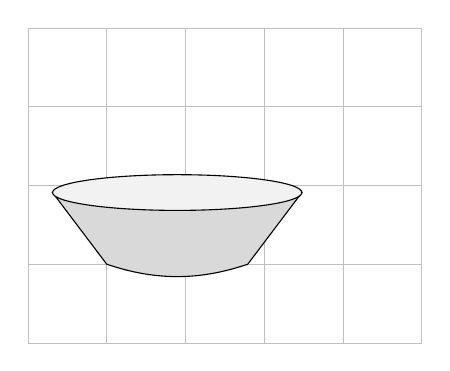
\begin{tikzpicture}

\pgfmathsetmacro{\acoor}{1.95 + random(1,3)*rnd}
\pgfmathsetmacro{\bcoor}{\acoor + rnd}
\pgfmathsetmacro{\ccoor}{.5 + .5*\acoor}
\pgfmathsetmacro{\first}{1 + (.4*\acoor - .5)}
\pgfmathsetmacro{\second}{1 + (.6*\acoor - .5)}
\pgfmathsetmacro{\split}{(2*\bcoor - 1 - \acoor)/2}
\pgfmathsetmacro{\ycoor}{1.5 + 2*rnd}
\pgfmathsetmacro{\corr}{.075 * \ycoor}
\pgfmathsetmacro{\abcorr}{(.08*(\bcoor - 1)) + .0065* \ycoor}


\draw [help lines,lightgray] (0,0) grid (5,4) ;
\draw[fill=gray!30] (1,1) .. controls (\first,1 - \abcorr) and (\second,1 - \abcorr) .. (\acoor,1) -- (\bcoor,\ycoor) --  (1 + \acoor - \bcoor,\ycoor) -- (1,1) ;
\draw[fill=gray!10] (\ccoor,\ycoor) ellipse (\split cm and \split*\corr cm) ;

\end{tikzpicture}
}

}
\newsavebox{\seventeen}
\savebox{\seventeen}{

\scalebox{4}{

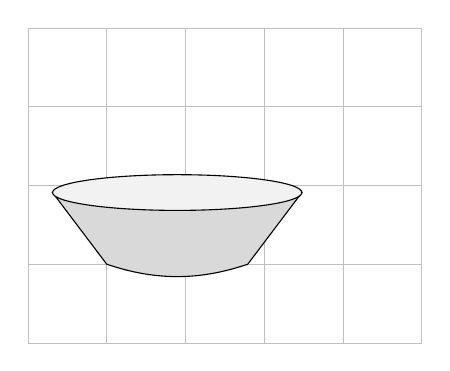
\begin{tikzpicture}

\pgfmathsetmacro{\acoor}{1.95 + random(1,3)*rnd}
\pgfmathsetmacro{\bcoor}{\acoor + rnd}
\pgfmathsetmacro{\ccoor}{.5 + .5*\acoor}
\pgfmathsetmacro{\first}{1 + (.4*\acoor - .5)}
\pgfmathsetmacro{\second}{1 + (.6*\acoor - .5)}
\pgfmathsetmacro{\split}{(2*\bcoor - 1 - \acoor)/2}
\pgfmathsetmacro{\ycoor}{1.5 + 2*rnd}
\pgfmathsetmacro{\corr}{.075 * \ycoor}
\pgfmathsetmacro{\abcorr}{(.08*(\bcoor - 1)) + .0065* \ycoor}


\draw [help lines,lightgray] (0,0) grid (5,4) ;
\draw[fill=gray!30] (1,1) .. controls (\first,1 - \abcorr) and (\second,1 - \abcorr) .. (\acoor,1) -- (\bcoor,\ycoor) --  (1 + \acoor - \bcoor,\ycoor) -- (1,1) ;
\draw[fill=gray!10] (\ccoor,\ycoor) ellipse (\split cm and \split*\corr cm) ;

\end{tikzpicture}
}

}
\newsavebox{\eightteen}
\savebox{\eightteen}{

\scalebox{4}{

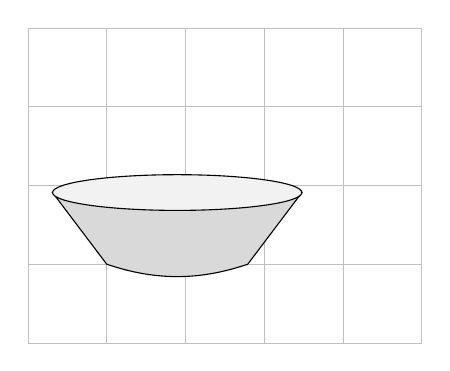
\begin{tikzpicture}

\pgfmathsetmacro{\acoor}{1.95 + random(1,3)*rnd}
\pgfmathsetmacro{\bcoor}{\acoor + rnd}
\pgfmathsetmacro{\ccoor}{.5 + .5*\acoor}
\pgfmathsetmacro{\first}{1 + (.4*\acoor - .5)}
\pgfmathsetmacro{\second}{1 + (.6*\acoor - .5)}
\pgfmathsetmacro{\split}{(2*\bcoor - 1 - \acoor)/2}
\pgfmathsetmacro{\ycoor}{1.5 + 2*rnd}
\pgfmathsetmacro{\corr}{.075 * \ycoor}
\pgfmathsetmacro{\abcorr}{(.08*(\bcoor - 1)) + .0065* \ycoor}


\draw [help lines,lightgray] (0,0) grid (5,4) ;
\draw[fill=gray!30] (1,1) .. controls (\first,1 - \abcorr) and (\second,1 - \abcorr) .. (\acoor,1) -- (\bcoor,\ycoor) --  (1 + \acoor - \bcoor,\ycoor) -- (1,1) ;
\draw[fill=gray!10] (\ccoor,\ycoor) ellipse (\split cm and \split*\corr cm) ;

\end{tikzpicture}
}

}
\newsavebox{\nineteen}
\savebox{\nineteen}{

\scalebox{4}{

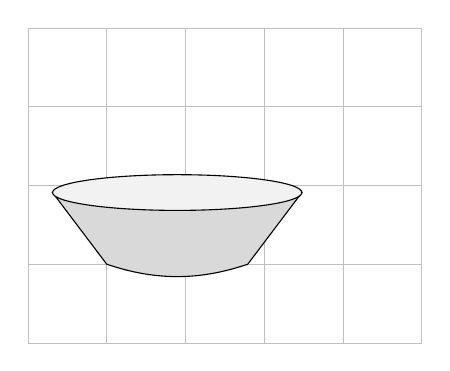
\begin{tikzpicture}

\pgfmathsetmacro{\acoor}{1.95 + random(1,3)*rnd}
\pgfmathsetmacro{\bcoor}{\acoor + rnd}
\pgfmathsetmacro{\ccoor}{.5 + .5*\acoor}
\pgfmathsetmacro{\first}{1 + (.4*\acoor - .5)}
\pgfmathsetmacro{\second}{1 + (.6*\acoor - .5)}
\pgfmathsetmacro{\split}{(2*\bcoor - 1 - \acoor)/2}
\pgfmathsetmacro{\ycoor}{1.5 + 2*rnd}
\pgfmathsetmacro{\corr}{.075 * \ycoor}
\pgfmathsetmacro{\abcorr}{(.08*(\bcoor - 1)) + .0065* \ycoor}


\draw [help lines,lightgray] (0,0) grid (5,4) ;
\draw[fill=gray!30] (1,1) .. controls (\first,1 - \abcorr) and (\second,1 - \abcorr) .. (\acoor,1) -- (\bcoor,\ycoor) --  (1 + \acoor - \bcoor,\ycoor) -- (1,1) ;
\draw[fill=gray!10] (\ccoor,\ycoor) ellipse (\split cm and \split*\corr cm) ;

\end{tikzpicture}
}

}
\newsavebox{\twenty}
\savebox{\twenty}{

\scalebox{4}{

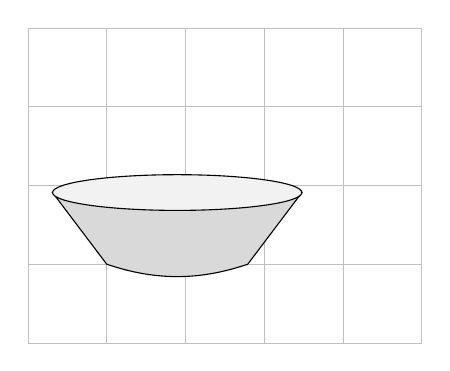
\begin{tikzpicture}

\pgfmathsetmacro{\acoor}{1.95 + random(1,3)*rnd}
\pgfmathsetmacro{\bcoor}{\acoor + rnd}
\pgfmathsetmacro{\ccoor}{.5 + .5*\acoor}
\pgfmathsetmacro{\first}{1 + (.4*\acoor - .5)}
\pgfmathsetmacro{\second}{1 + (.6*\acoor - .5)}
\pgfmathsetmacro{\split}{(2*\bcoor - 1 - \acoor)/2}
\pgfmathsetmacro{\ycoor}{1.5 + 2*rnd}
\pgfmathsetmacro{\corr}{.075 * \ycoor}
\pgfmathsetmacro{\abcorr}{(.08*(\bcoor - 1)) + .0065* \ycoor}


\draw [help lines,lightgray] (0,0) grid (5,4) ;
\draw[fill=gray!30] (1,1) .. controls (\first,1 - \abcorr) and (\second,1 - \abcorr) .. (\acoor,1) -- (\bcoor,\ycoor) --  (1 + \acoor - \bcoor,\ycoor) -- (1,1) ;
\draw[fill=gray!10] (\ccoor,\ycoor) ellipse (\split cm and \split*\corr cm) ;

\end{tikzpicture}
}

}
\newsavebox{\twentyone}
\savebox{\twentyone}{

\scalebox{4}{

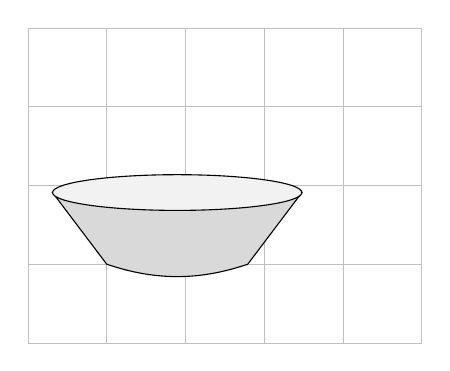
\begin{tikzpicture}

\pgfmathsetmacro{\acoor}{1.95 + random(1,3)*rnd}
\pgfmathsetmacro{\bcoor}{\acoor + rnd}
\pgfmathsetmacro{\ccoor}{.5 + .5*\acoor}
\pgfmathsetmacro{\first}{1 + (.4*\acoor - .5)}
\pgfmathsetmacro{\second}{1 + (.6*\acoor - .5)}
\pgfmathsetmacro{\split}{(2*\bcoor - 1 - \acoor)/2}
\pgfmathsetmacro{\ycoor}{1.5 + 2*rnd}
\pgfmathsetmacro{\corr}{.075 * \ycoor}
\pgfmathsetmacro{\abcorr}{(.08*(\bcoor - 1)) + .0065* \ycoor}


\draw [help lines,lightgray] (0,0) grid (5,4) ;
\draw[fill=gray!30] (1,1) .. controls (\first,1 - \abcorr) and (\second,1 - \abcorr) .. (\acoor,1) -- (\bcoor,\ycoor) --  (1 + \acoor - \bcoor,\ycoor) -- (1,1) ;
\draw[fill=gray!10] (\ccoor,\ycoor) ellipse (\split cm and \split*\corr cm) ;

\end{tikzpicture}
}

}
\newsavebox{\twentytwo}
\savebox{\twentytwo}{

\scalebox{4}{

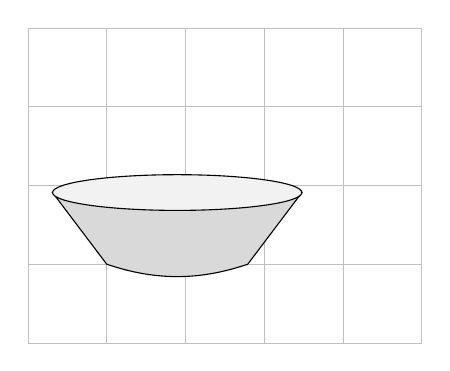
\begin{tikzpicture}

\pgfmathsetmacro{\acoor}{1.95 + random(1,3)*rnd}
\pgfmathsetmacro{\bcoor}{\acoor + rnd}
\pgfmathsetmacro{\ccoor}{.5 + .5*\acoor}
\pgfmathsetmacro{\first}{1 + (.4*\acoor - .5)}
\pgfmathsetmacro{\second}{1 + (.6*\acoor - .5)}
\pgfmathsetmacro{\split}{(2*\bcoor - 1 - \acoor)/2}
\pgfmathsetmacro{\ycoor}{1.5 + 2*rnd}
\pgfmathsetmacro{\corr}{.075 * \ycoor}
\pgfmathsetmacro{\abcorr}{(.08*(\bcoor - 1)) + .0065* \ycoor}


\draw [help lines,lightgray] (0,0) grid (5,4) ;
\draw[fill=gray!30] (1,1) .. controls (\first,1 - \abcorr) and (\second,1 - \abcorr) .. (\acoor,1) -- (\bcoor,\ycoor) --  (1 + \acoor - \bcoor,\ycoor) -- (1,1) ;
\draw[fill=gray!10] (\ccoor,\ycoor) ellipse (\split cm and \split*\corr cm) ;

\end{tikzpicture}
}

}
\newsavebox{\twentythree}
\savebox{\twentythree}{

\scalebox{4}{

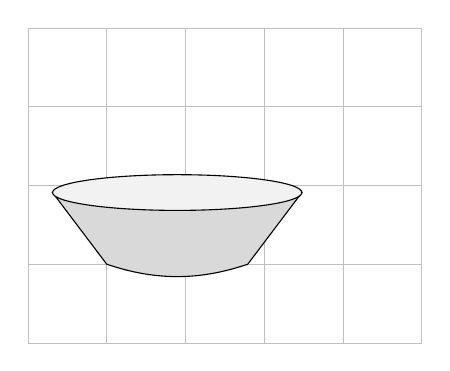
\begin{tikzpicture}

\pgfmathsetmacro{\acoor}{1.95 + random(1,3)*rnd}
\pgfmathsetmacro{\bcoor}{\acoor + rnd}
\pgfmathsetmacro{\ccoor}{.5 + .5*\acoor}
\pgfmathsetmacro{\first}{1 + (.4*\acoor - .5)}
\pgfmathsetmacro{\second}{1 + (.6*\acoor - .5)}
\pgfmathsetmacro{\split}{(2*\bcoor - 1 - \acoor)/2}
\pgfmathsetmacro{\ycoor}{1.5 + 2*rnd}
\pgfmathsetmacro{\corr}{.075 * \ycoor}
\pgfmathsetmacro{\abcorr}{(.08*(\bcoor - 1)) + .0065* \ycoor}


\draw [help lines,lightgray] (0,0) grid (5,4) ;
\draw[fill=gray!30] (1,1) .. controls (\first,1 - \abcorr) and (\second,1 - \abcorr) .. (\acoor,1) -- (\bcoor,\ycoor) --  (1 + \acoor - \bcoor,\ycoor) -- (1,1) ;
\draw[fill=gray!10] (\ccoor,\ycoor) ellipse (\split cm and \split*\corr cm) ;

\end{tikzpicture}
}

}
\newsavebox{\twentyfour}
\savebox{\twentyfour}{

\scalebox{4}{

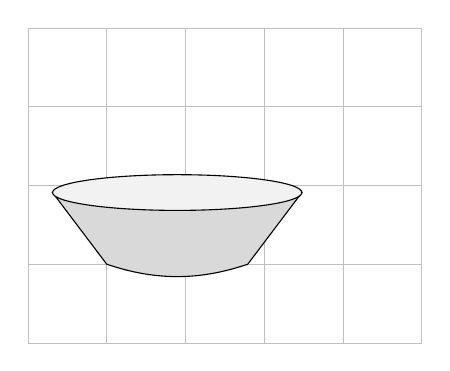
\begin{tikzpicture}

\pgfmathsetmacro{\acoor}{1.95 + random(1,3)*rnd}
\pgfmathsetmacro{\bcoor}{\acoor + rnd}
\pgfmathsetmacro{\ccoor}{.5 + .5*\acoor}
\pgfmathsetmacro{\first}{1 + (.4*\acoor - .5)}
\pgfmathsetmacro{\second}{1 + (.6*\acoor - .5)}
\pgfmathsetmacro{\split}{(2*\bcoor - 1 - \acoor)/2}
\pgfmathsetmacro{\ycoor}{1.5 + 2*rnd}
\pgfmathsetmacro{\corr}{.075 * \ycoor}
\pgfmathsetmacro{\abcorr}{(.08*(\bcoor - 1)) + .0065* \ycoor}


\draw [help lines,lightgray] (0,0) grid (5,4) ;
\draw[fill=gray!30] (1,1) .. controls (\first,1 - \abcorr) and (\second,1 - \abcorr) .. (\acoor,1) -- (\bcoor,\ycoor) --  (1 + \acoor - \bcoor,\ycoor) -- (1,1) ;
\draw[fill=gray!10] (\ccoor,\ycoor) ellipse (\split cm and \split*\corr cm) ;

\end{tikzpicture}
}

}
\newsavebox{\twentyfive}
\savebox{\twentyfive}{

\scalebox{4}{

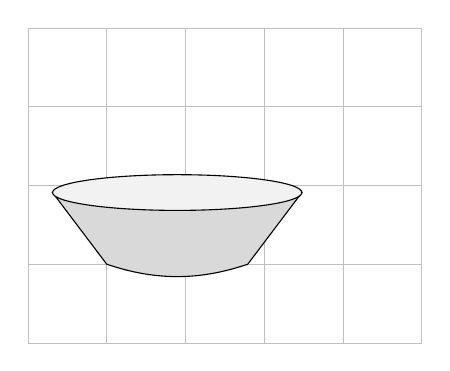
\begin{tikzpicture}

\pgfmathsetmacro{\acoor}{1.95 + random(1,3)*rnd}
\pgfmathsetmacro{\bcoor}{\acoor + rnd}
\pgfmathsetmacro{\ccoor}{.5 + .5*\acoor}
\pgfmathsetmacro{\first}{1 + (.4*\acoor - .5)}
\pgfmathsetmacro{\second}{1 + (.6*\acoor - .5)}
\pgfmathsetmacro{\split}{(2*\bcoor - 1 - \acoor)/2}
\pgfmathsetmacro{\ycoor}{1.5 + 2*rnd}
\pgfmathsetmacro{\corr}{.075 * \ycoor}
\pgfmathsetmacro{\abcorr}{(.08*(\bcoor - 1)) + .0065* \ycoor}


\draw [help lines,lightgray] (0,0) grid (5,4) ;
\draw[fill=gray!30] (1,1) .. controls (\first,1 - \abcorr) and (\second,1 - \abcorr) .. (\acoor,1) -- (\bcoor,\ycoor) --  (1 + \acoor - \bcoor,\ycoor) -- (1,1) ;
\draw[fill=gray!10] (\ccoor,\ycoor) ellipse (\split cm and \split*\corr cm) ;

\end{tikzpicture}
}

}

\newsavebox{\twentysix}
\savebox{\twentysix}{

\scalebox{4}{

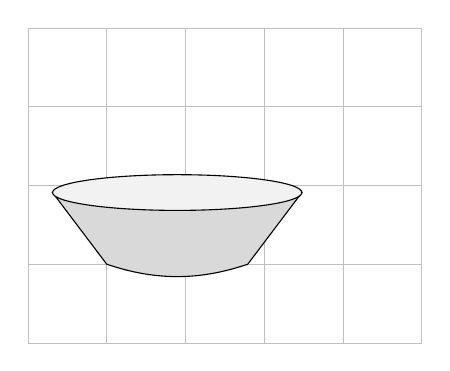
\begin{tikzpicture}

\pgfmathsetmacro{\acoor}{1.95 + random(1,3)*rnd}
\pgfmathsetmacro{\bcoor}{\acoor + rnd}
\pgfmathsetmacro{\ccoor}{.5 + .5*\acoor}
\pgfmathsetmacro{\first}{1 + (.4*\acoor - .5)}
\pgfmathsetmacro{\second}{1 + (.6*\acoor - .5)}
\pgfmathsetmacro{\split}{(2*\bcoor - 1 - \acoor)/2}
\pgfmathsetmacro{\ycoor}{1.5 + 2*rnd}
\pgfmathsetmacro{\corr}{.075 * \ycoor}
\pgfmathsetmacro{\abcorr}{(.08*(\bcoor - 1)) + .0065* \ycoor}


\draw [help lines,lightgray] (0,0) grid (5,4) ;
\draw[fill=gray!30] (1,1) .. controls (\first,1 - \abcorr) and (\second,1 - \abcorr) .. (\acoor,1) -- (\bcoor,\ycoor) --  (1 + \acoor - \bcoor,\ycoor) -- (1,1) ;
\draw[fill=gray!10] (\ccoor,\ycoor) ellipse (\split cm and \split*\corr cm) ;

\end{tikzpicture}
}

}


%%%%%%%%%%%%%%%%%%%%%%%%%%%%%%%%%%%%%%%%%

\newpage

\begin{landscape}

\begin{picture}(250,250)
	\put(-50,-150){\usebox{\one}}
\end{picture}

\end{landscape}

\newpage

\begin{landscape}

\begin{picture}(250,250)
	\put(-50,-150){\usebox{\two}}
\end{picture}

\end{landscape}

\newpage

\begin{landscape}

\begin{picture}(250,250)
	\put(-50,-150){\usebox{\three}}
\end{picture}

\end{landscape}

\newpage

\begin{landscape}

\begin{picture}(250,250)
	\put(-50,-150){\usebox{\four}}
\end{picture}

\end{landscape}

\newpage

\begin{landscape}

\begin{picture}(250,250)
	\put(-50,-150){\usebox{\five}}
\end{picture}

\end{landscape}

\newpage

\begin{landscape}

\begin{picture}(250,250)
	\put(-50,-150){\usebox{\six}}
\end{picture}

\end{landscape}

\newpage

\begin{landscape}

\begin{picture}(250,250)
	\put(-50,-150){\usebox{\seven}}
\end{picture}

\end{landscape}

\newpage

\begin{landscape}

\begin{picture}(250,250)
	\put(-50,-150){\usebox{\eight}}
\end{picture}

\end{landscape}

\newpage

\begin{landscape}

\begin{picture}(250,250)
	\put(-50,-150){\usebox{\nine}}
\end{picture}

\end{landscape}

\newpage

\begin{landscape}

\begin{picture}(250,250)
	\put(-50,-150){\usebox{\ten}}
\end{picture}

\end{landscape}

\newpage

\begin{landscape}

\begin{picture}(250,250)
	\put(-50,-150){\usebox{\eleven}}
\end{picture}

\end{landscape}

\newpage

\begin{landscape}

\begin{picture}(250,250)
	\put(-50,-150){\usebox{\twelve}}
\end{picture}

\end{landscape}

\newpage

\begin{landscape}

\begin{picture}(250,250)
	\put(-50,-150){\usebox{\thirteen}}
\end{picture}

\end{landscape}

\newpage

\begin{landscape}

\begin{picture}(250,250)
	\put(-50,-150){\usebox{\fourteen}}
\end{picture}

\end{landscape}

\newpage

\begin{landscape}

\begin{picture}(250,250)
	\put(-50,-150){\usebox{\fifteen}}
\end{picture}

\end{landscape}

\newpage

\begin{landscape}

\begin{picture}(250,250)
	\put(-50,-150){\usebox{\sixteen}}
\end{picture}

\end{landscape}

\newpage

\begin{landscape}

\begin{picture}(250,250)
	\put(-50,-150){\usebox{\seventeen}}
\end{picture}

\end{landscape}

\newpage

\begin{landscape}

\begin{picture}(250,250)
	\put(-50,-150){\usebox{\eightteen}}
\end{picture}

\end{landscape}

\newpage

\begin{landscape}

\begin{picture}(250,250)
	\put(-50,-150){\usebox{\nineteen}}
\end{picture}

\end{landscape}

\newpage

\begin{landscape}

\begin{picture}(250,250)
	\put(-50,-150){\usebox{\twenty}}
\end{picture}

\end{landscape}

\newpage

\begin{landscape}

\begin{picture}(250,250)
	\put(-50,-150){\usebox{\twentyone}}
\end{picture}

\end{landscape}

\newpage

\begin{landscape}

\begin{picture}(250,250)
	\put(-50,-150){\usebox{\twentytwo}}
\end{picture}

\end{landscape}

\newpage

\begin{landscape}

\begin{picture}(250,250)
	\put(-50,-150){\usebox{\twentythree}}
\end{picture}

\end{landscape}

\newpage

\begin{landscape}

\begin{picture}(250,250)
	\put(-50,-150){\usebox{\twentyfour}}
\end{picture}

\end{landscape}

\newpage

\begin{landscape}

\begin{picture}(250,250)
	\put(-50,-150){\usebox{\twentyfive}}
\end{picture}

\end{landscape}

\newpage

\begin{landscape}

\begin{picture}(250,250)
	\put(-50,-150){\usebox{\twentysix}}
\end{picture}

\end{landscape}


\end{document}
